\section{Boosting}
Nach meiner eigenen Erfahrung als Student fällt oft auf, dass Gruppenarbeit nicht immer die erwarteten Vorteile bringt. Oft dominiert in Lerngruppen ein einzelner Student, der über fundiertes Wissen verfügt, die Diskussion und die Gruppenleistung spiegelt im Wesentlichen seine individuelle Leistung wider. 
\newline
In Fällen, wo alle Mitglieder einer Lerngruppe nur begrenztes Wissen zu einem Thema haben, kann die kollektive Leistung sogar hinter dem zurückbleiben, was man durch zufällige Antworten erwarten würde. Die Vorstellung, dass eine Gruppe von Individuen mit begrenztem Wissen gemeinsam Ergebnisse erzielen kann, die sowohl den Durchschnitt als auch jede individuelle Bestleistung übertreffen, widerspricht oft unserer Intuition. Selbst historische Weisheiten, wie sie in der Bibel gefunden werden, betonen die Risiken einer solchen Zusammenarbeit. Dort heißt es metaphorisch: ``Wenn aber ein Blinder den andern führt, so fallen sie beide in die Grube'' (Mt 23,16; Mt 23,24; Lk 6,39; Röm 2,19).
\newline
\newline
Doch im Bereich des maschinellen Lernens offenbart sich ein ganz anderes Szenario. Hier ermöglicht das Boosting-Verfahren, dass die Kombination von schwachen Modellen zu einem leistungsstarken Gesamtsystem führt. Dieser Ansatz, der die aggregierte Intelligenz mehrerer einfacher Modelle nutzt, um komplexe Probleme zu lösen, steht im starken Gegensatz zu den oft enttäuschenden Ergebnissen menschlicher Gruppenarbeit mit begrenztem Wissen \cite[S.~3]{SchapireFreund2012}.

\subsection{Was ist Boosting}
\begin{mdframed}
    \textbf{Boosting (ursprünglich Hypothesis Boosting)} bezeichnet eine beliebige Ensemble-Methode des Supervised Learning, bei der sich mehrere schwache Lerner durch Hintereinanderausführung (iterativ) zu einem starken Lerner kombinieren lassen. \textcite[S.~191]{Geron2018}. Das Boosting findet statt, indem die Fehler des Vorgängers stark höher gewichtet werden für die folgende Lerniteration als richtig erkannte Zuordnungen. So beschäftigt sich jede Lerninstanz primär mit der Ausmerzung der Fehler des Vorgängers.
    
Es gibt eine entfernte Verwandtschaft des Boostings zu der "Attention" in modernen Transformer-Architekturen wie GPT. Der meist verwendete Gradientenabstieg zur Fehlerminimierung in Boosting-Verfahren ähnelt wiederum den auch in Neuronalen Netzen verwendeten Gradientenabstiegsverfahren wie z.B. Backpropagation. Ein Unterschied sind jedoch meist wesentlich geringer benötigte Ressourcen und Lernzeiten als bei Deep Learning Modellen, wo sehr hohe Zahlen von Parametern nötig sind.

Zu einem bekannten anderen Verfahren des Ensemble Learning, den Random Forests besteht ein grundsätzlicher Unterschied: Random Forests sind **parallele** Lerninstanzen, deren Ergebnisse kombiniert werden, z.B. durch Mehrheitsentscheide, wohingegen Boosting Verfahren prinzipiell **sequentiell** ausgeführt werden, weil ja auf den Fehler des Vorgängers abgestellt wird. Andere Parallelisierungen sind natürlich möglich.\textcite[S.343]{Frochte202} Insbesondere können natürlich auch beim Boosting mehrere Klassifikatoren parallel betrachtet und kombiniert werden.

\subsection{Beispiel Wettererkennung}
\end{mdframed}

Die genannte Definition des Boosting lässt sich gut anhand des Beispiels der Wettererkennung veranschaulichen. Betrachten wir folgende einfache Regeln (Schwache Lerner) zur Beurteilung, ob es regnet:

\begin{table}[h]
    \centering
    \begin{tabular}{|l|l|}
    \hline
    \textbf{Schwache Lerner}      & \textbf{Grenzwert}   \\ \hline
    Nasser Boden               & Ja                  \\ \hline
    Wolken am Himmel           & Ja                  \\ \hline
    Hohe Luftfeuchtigkeit      & $>$ 80\%             \\ \hline
    Personen mit Regenschirm   & Ja                  \\ \hline
    Außentemperatur            & $>$ 0°C             \\ \hline
    \end{tabular}
    \caption{Individuelle Vorhersagen der Schwache Lerner}
    \label{tab:weak_learners}
\end{table}

Beispielsweise ist ein nasser Boden zwar eine Voraussetzung und ein guter erster Filter, allerdings könnte der Boden genauso gut durch einen Rasensprenger nass sein.
\newline
Die Temperatur ist hingegen ein relativ schlechtes Indiz für die Frage, ob es gerade regnet. Es unterscheidet aber den Fall Regen und Schnee und ist somit trotzdem essentiell für die Klassifikation.

\subsubsection{Erzeugung eines starken Lerners}
Der nächste Schritt ist es, die Aussagen der schwachen Lerner in ein nützliches Model zusammenzufassen, einen sog. `starken Lerner'. Im einfachsten Fall lässt man die schwachen Lerner mit gleicher Stimmkraft abstimmen. Aus dem Stimmverhältnis der Vorhersagen der schwachen Lerner lässt sich in unserem Fall die Regenwahrscheinlichkeit ableiten.

\begin{table}[h]
    \centering
    \begin{tabular}{|l|l|l|l|l|l|}
    \hline
    Nasser Boden & Wolken & Hohe Luftfeuchte & Regenschirm & Über 0°C & Regenwahrscheinlichkeit (\%) \\ \hline
    Ja & Ja & Ja & Ja & Ja & 100\% \\ \hline
    Ja & Ja & Nein & Nein & Ja & 60\% \\ \hline
    Nein & Ja & Ja & Ja & Ja & 80\% \\ \hline
    Ja & Nein & Ja & Nein & Ja & 60\% \\ \hline
    Nein & Nein & Nein & Nein & Ja & 20\% \\ \hline
    Ja & Ja & Ja & Nein & Nein & 60\% \\ \hline
    Nein & Ja & Nein & Ja & Ja & 80\% \\ \hline
    ... & ... & ... & ... & ... & ... \\ \hline
    \end{tabular}
    \caption{Wahrheitstabelle zur Vorhersage von Regen basierend auf schwachen Lernern. Die Werte dienen in erster Linie der Veranschaulichung.}
    \label{tab:rain_prediction}
\end{table}

\subsection{Gewichtete Abstimmung}
Aus der Mehrheitsentscheidung, bei der alle schwachen Lerner die gleiche Stimmkraft haben, eine Vorhersage zu treffen, liefert nur selten die besten Ergebnisse. Eine bessere Vorgehensweise, die auch von vielen Boosting-Algorithmen benutzt wird, ist die gewichtete Abstimmung. Diese Methode berechnet die Stimmkraft oder Gewichtung des Lerners \( \alpha \) individuell, wie im Algorithmus 1.1 von Schapire und Freund beschrieben \parencite[S.~5]{SchapireFreund2012}.

\subsubsection{Grundlegende Annahmen}
\begin{mdframed}
    \textbf{Gegeben:} \\
    - Ein Datensatz \( X \), bestehend aus \( n \) Beispielpaaren, wobei jedes Paar aus einem Eingabedatum \( x_i \) und dem entsprechenden Zielwert \( y_i \) besteht: \( X = \{(x_1, y_1), (x_2, y_2), \dots, (x_n, y_n)\} \). \\
    - Schwache Lerner \( t \) mit Vorhersagefunktion/Hypthese \( h_t \).
\end{mdframed}

Jeder schwache Lerner trifft Vorhersagen basierend auf dem Datensatz \( X \). Der Erfolg dieser Vorhersagen wird durch den Fehler \( \varepsilon_t \) gemessen.

\subsubsection{Fehlerberechnung}\label{sec:errorComputation}
Der Fehler \( \varepsilon_t \) eines schwachen Lerners ist der Anteil der falschen Vorhersagen:
\begin{gather}
    \varepsilon_t = \frac{1}{n} \sum_{i=1}^{n} \mathbb{I}(h_t(x_i) \neq y_i),
\end{gather}
wobei \( \mathbb{I} \) die Indikatorfunktion ist, die 1 ist, wenn \( h_t(x_i) \neq y_i \) (d.h., die Vorhersage ist falsch), und 0 sonst.

\subsubsection{Gewichtung der schwachen Lerner}\label{sec:weightedLearners}
Die Gewichtung \( \alpha_t \) jedes schwachen Lerners basiert auf seinem Fehler \( \varepsilon_t \):
\begin{gather}
    \alpha_t = \ln\left(\frac{1 - \varepsilon_t}{\varepsilon_t}\right).
\end{gather}
Ein zuverlässiger Lerner \( t \) hat eine höhere Gewichtung \( \alpha_t \) je nach dem wie groß sein Fehler \( \varepsilon_t \) ist.

\begin{figure}[h]
    \centering
    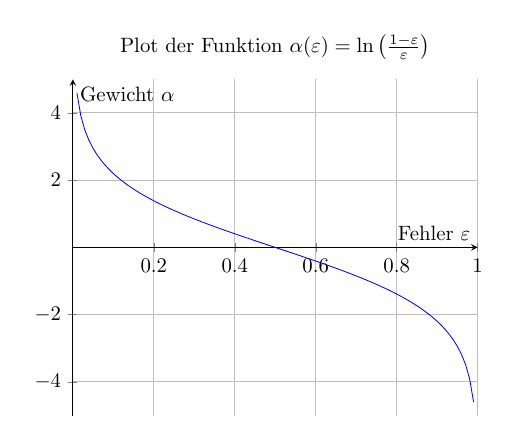
\begin{tikzpicture}[scale=0.75]
    \begin{axis}[
        title={Plot der Funktion \( \alpha(\varepsilon) = \ln\left(\frac{1 - \varepsilon}{\varepsilon}\right) \)},
        xlabel={Fehler \( \varepsilon \)},
        ylabel={Gewicht \( \alpha \)},
        xmin=0, xmax=1,
        ymin=-5, ymax=5,
        grid=both,
        axis lines=middle
    ]
    
    \addplot[
        domain=0.01:0.99, 
        samples=100, 
        color=blue,
    ]
    {ln((1-x)/x)};
    \end{axis}
    \end{tikzpicture}
    \caption{Visualisierung der Gewichtsfunktion \( \alpha \) in Abhängigkeit vom Fehler \( \varepsilon \)}
    \label{fig:alpha_plot}
\end{figure}
    

\subsubsection{Endgültige Vorhersage des starken Lerners}
Die Gesamtvorhersage \( H \) des Boosting-Modells ergibt sich aus der gewichteten Abstimmung aller schwachen Lerner.

\begin{equation}
    H(x) = \text{sign}\left(\sum_{t=1}^{T} \alpha_t h_t(x)\right).
\end{equation}
    
In anderen Worten wird die Vorhersage eines Lerners auf den Daten \( h_t(x) \) mit seiner Gewichtung \( \alpha \) multipliziert. Die Summe dieses Produkts für alle Lerner \( T \) ergibt die Gesamtvorhersage \( H \). Hier wird lediglich noch die Signum-Funktion angewendet, um den Wert zwischen 0 und 1 zu glätten.

% Plot der Signum-Funktion
\begin{figure}[h]
    \centering
    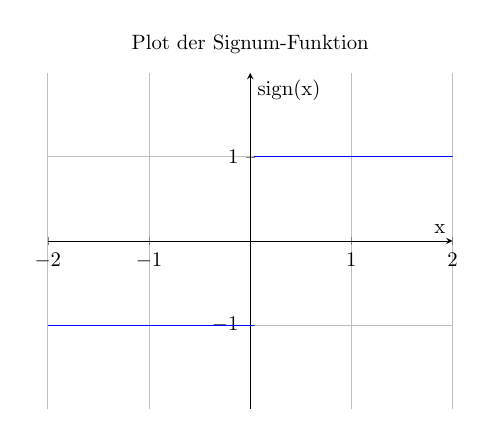
\begin{tikzpicture}[scale=0.75]
    \begin{axis}[
        title={Plot der Signum-Funktion},
        xlabel={x},
        ylabel={sign(x)},
        xmin=-2, xmax=2,
        ymin=-2, ymax=2,
        grid=both,
        axis lines=middle,
        ytick={-1,0,1},
        xtick={-2,-1,0,1,2}
    ]
    
    \addplot[
        domain=-2:2, 
        samples=50, 
        color=blue,
        jump mark left,
    ]
    {sign(x)};
    
    \end{axis}
    \end{tikzpicture}
    \caption{Visualisierung der Signum-Funktion}
    \label{fig:signum_function}
\end{figure}

\subsection{Annahme des schwache Lernens}
\label{sec:assumptionOfWeakLearning}
Die Voraussetzung jedes Boosting-Algorithmus ist ein bereits vorhandener schwacher Basis-Lernalgorithmus. Das Ziel ist es dann, durch mehrfache Ausführung des Boosting-Algorithmus' die Leistung des Lernalgorithmus zu verbessern, bzw. zu `boosten'. Laut \textcite[S. S.~4]{SchapireFreund2012} reicht es aus geringe Ansprüche an die Leistung der schwachen Lerner zu stellen. Es ist völlig hinreichend, wenn der Lernalgorithmus Hypothesen liefert mit etwas besseren Ergebnissen als 50\% Fehlerquote, was dem uninformierten Raten gleich käme.
\newline
Diese Annahme, dass der Lerner schwache Hypothesen hervorbringt, die mindestens etwas besser sind als zufälliges Raten, wird die \textit{Annahme des schwachen Lernens genannt}.